%%%%%%%%%%%%%%%%%% BUNDLES AND CONNECTION

\chapter{Bundles and Connections}

So far, tangent and cotangent bundles have been considered, and other generalisations have been slightly appearing.

Instead of attacking the problem formally, in the following, a heuristic introduction to more general bundles is shown, and also the definition of connections on these bundles.

\section{Fibre Bundles}

A bundle is a geometric structure composed by two manifolds $E$ (the bundle) and $M$ (the base)\footnote{In some sense the base manifold is a ``piece'' of the bundle, i.e., $M\subset E$.} together with a projection map $\pi:E\to M$. If $U\subset M$, then locally, $E\simeq U\times F$, where $F$ is a manifold called the fibre of $E$. 

\subsubsection*{Examples}
\begin{itemize}
\item A cylinder is a bundle $E$ with base manifold $M=\R$ and fibre $F=S^1$, s.t. $\pi:\R\times S^1\to \R$.
  
  In this case, $E=M\times F$ globally, then the bundle is called {\sc Trivial}.
\item If one takes an interval $I\subset \R$, the ``finite'' cylinder is a trivial bundle $E=I\times S^1$ or $E=S^1\times I$.
  %% \begin{center}
  %%   \begin{tikzpicture}[rotate=90]
      
  %%     \begin{axis}[
  %%         hide axis,
  %%         view={40}{40}
  %%       ]
  %%       \addplot3 [
  %%         surf, shader=faceted interp,
  %%         point meta=x,
  %%         colormap/greenyellow,
  %%         samples=40,
  %%         samples y=5,
  %%         z buffer=sort,
  %%         domain=0:360,
  %%         y domain=-0.5:0.5
  %%       ] (
  %%                 {cos(x)},
  %%                 {sin(x)},
  %%                 {0.5*y});
  %%       \addplot3 coordinates {(0,0,-3) (0,3,0)};
  %%     \end{axis}
  %%   \end{tikzpicture}
  %% \end{center}
\item The simplest non-trivial bundle is a M\"obius strip, which is a bundle $E$ locally homeomorphic to $S^1\times I$, but is not globally $S^1\times I$ because there is a ``twist'' (a bit more formally there is a $Z_2$-action on the fibre).
  \begin{center}
    %\tikzsetnextfilename{CylinderMoebius}
    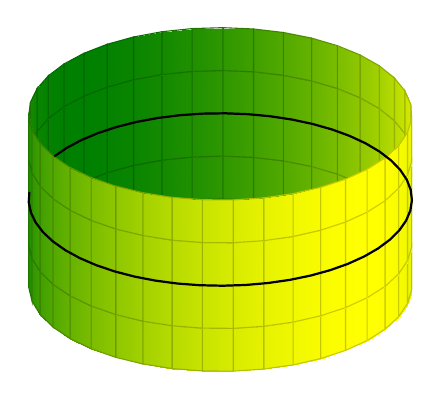
\begin{tikzpicture}
      \begin{axis}[
          hide axis,
          view={40}{40}
        ]
        \addplot3 [
          surf, shader=faceted interp,
          point meta=x,
          colormap/greenyellow,
          samples=40,
          samples y=5,
          z buffer=sort,
          domain=0:360,
          y domain=-0.5:0.5
        ] (
                  {cos(x)},
                  {sin(x)},
                  {0.5*y});
        \addplot3 [
          samples=50,
          domain=-145:190, % The domain needs to be adjusted manually, depending on the camera angle, unfortunately
          samples y=0,
          thick
        ] (
                  {cos(x)},
                  {sin(x)},
                  {0}); 
      \end{axis}
      \end{tikzpicture}
      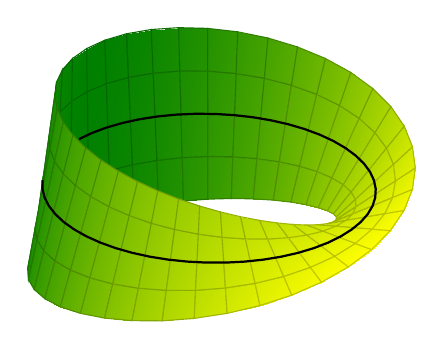
\begin{tikzpicture}
      \begin{axis}[
          hide axis,
          view={40}{40}
        ]
        \addplot3 [
          surf, shader=faceted interp,
          point meta=x,
          colormap/greenyellow,
          samples=40,
          samples y=5,
          z buffer=sort,
          domain=0:360,
          y domain=-0.5:0.5
        ] (
                  {(1+0.5*y*cos(x/2))*cos(x)},
                  {(1+0.5*y*cos(x/2))*sin(x)},
                  {0.5*y*sin(x/2)});
        \addplot3 [
          samples=50,
          domain=-145:180, % The domain needs to be adjusted manually, depending on the camera angle, unfortunately
          samples y=0,
          thick
        ] (
                  {cos(x)},
                  {sin(x)},
                  {0}); 
      \end{axis}
    \end{tikzpicture}
  \end{center}
\item  A 2-torus $T^2$ is a trivial bundle with base manifold $M=S^1$ and fibre $F=S^1$.
\end{itemize}

In essence there are three types of bundles:
\begin{description}
\item [Fibre Bundle] is a general bundle structure, i.e., a manifold which locally looks like a product of a base manifold and the fibre.
\item [Vector Bundle] A fibre bundle whose fibre is a vector space.
\item [Principal Bundle] A fibre bundle whose fibre is a manifold with group structure, i.e., the fibre is a lie group manifold.
\end{description}

\subsection{Sections on Bundles}

A section, $\psi$, on $E\xrightarrow{\pi}M$ is a smooth map from the base manifold to the fibre,
\begin{align}
  \psi:M\to F,
\end{align}
such that $\pi\circ\psi= \id_M$.

Sections are one important object for physicist, because they represent the physical fields of a theory.

\subsection{More About Principal Bundles}

As stated before, principal bundles are fibre bundles whose fibres are a Lie Group. Therefore, there is an action of $G$ on $F$. They are the natural framework for the study of Gauge Theories.

\subsubsection*{Associated Bundles}

The associated bundles are constructed from  principal bundles. Let $P(M,G)$ be a principal bundle, with fibre $F$ admitting and action of the Lie group $G$.

Given a pair $(u,f)$ on $P\times F$, a bundle $\(P\times F\)/G$ can be construct by identifying points related by the action of the group $G$, 
\begin{align}
  (u,f)\sim \(u g,g^{-1}f\).
\end{align}
This construction is known as {\sc Associated Bundle}.

More generally, the fibre can admit the action of a representation $\rho$ of $G$. In this case, the associated bundle $\(P\times_\rho F\)/G$ is constructed through,
\begin{align}
  (u,f)\sim \(u g,\rho\(g^{-1}\)f\).
\end{align}


\section{Connections on the Tangent Bundle}

A connection on the tangent bundle is an application $\nabla:TM\times TM\to TM$, defined by
\begin{align}
  \nabla:(X,Y)\to \nabla_X Y,
\end{align}
satisfying 
\begin{align}
  \nabla_{fX}Y &=f \nabla_X Y\\
  \nabla_X fY &= f\nabla_X Y+ Y . X[f],\\
  \nabla_{X+ Y} Z &= \nabla_X Z+\nabla_Y Z.
\end{align}

On a vector basis, 
\begin{align}
  \nabla_{\partial_i}\partial_j \equiv \nabla_i\partial_j = \conn{i}{k}{j}\pa{k},
\end{align}
then, in components
\begin{align}
  \nab{i}Y=\(\pa{i}Y^j+\conn{i}{j}{k}Y^k\)\pa{j}.
\end{align}
In physics, the term between the brackets is called the covariant derivative of a vector.


\begin{infobox}[frametitle={General Connections}]
  In a general bundle $E$, the connections are applications
  \begin{align*}
    \nabla:TM\otimes\mathcal{E}\to\mathcal{E},
  \end{align*}
  where $\mathcal{E}$ is the space of sections on the bundle $E$.
\end{infobox}

\section{Parallel Transport and Geodesic}

Let $V$ be a tangent vector to a curve, i.e., 
\begin{align}
  V=\frac{d x^\mu}{d t}\(c(t)\)\;\left.\pa{\mu}\right|_{c(t)},
\end{align}
then $X\in TM$ is said to be parallel transport along $c(t)$ if
\begin{align}
  \nabla_V X =0\quad \forall\;t\in I.
\end{align}

If the tangent vector to a curve ($V$) satisfies the parallel transport condition,
\begin{align}
  \nabla_V V =0,
\end{align}
then the curve $c(t)$ is called a {\sc Geodesic}.

\begin{Ebox}
  \begin{itemize}
  \item Use that
    \begin{align*}
      \nab{i}\pa{j} &=\conn{i}{k}{j}\pa{k}\\
      \nab{i}'\pa{j}' &=\(\Ga_{i}'\)^{k}{}_{j}\pa{k}',
    \end{align*}
    to find the transformation rule of $\Ga$'s.
  \item Find the action of $\nabla$ on 1-forms and rank two tensors.
  \item Write in coordinates the condition of parallel transport and geodesic curve.
  \end{itemize}
\end{Ebox}


\section{Torsion and Curvature}

\begin{align}
  T(X,Y) &= \nab{X}Y-\nab{Y}X-\comm{X}{Y}\\
  R(X,Y,Z) &= \nab{X}\nab{Y}Z -\nab{Y}\nab{X}Z -\nab{\comm{X}{Y}}Z.
\end{align}

\begin{Ebox}
  \begin{itemize}
  \item Find coordinate expressions for $T(X,Y)$ and $R(X,Y,Z)$.
  \item Show that they are multilinear objects, i.e., they are tensors.
  \end{itemize}
\end{Ebox}
\bigskip
\begin{infobox}[frametitle={NOTE}]
  In general the concept of curvature can be extended to sections on a bundle, where 
  \begin{align*}
    \nabla:TM\otimes\mathcal{E}\to\mathcal{E},
  \end{align*}
  while the torsion cannot, since $X$ and $Y$ are necessarily the same kind of object.
\end{infobox}


